\documentclass[main.tex]{subfiles}
\begin{document}
    \chapter{Electrical}
    \label{ch:electrical}

    \section{Battery}
      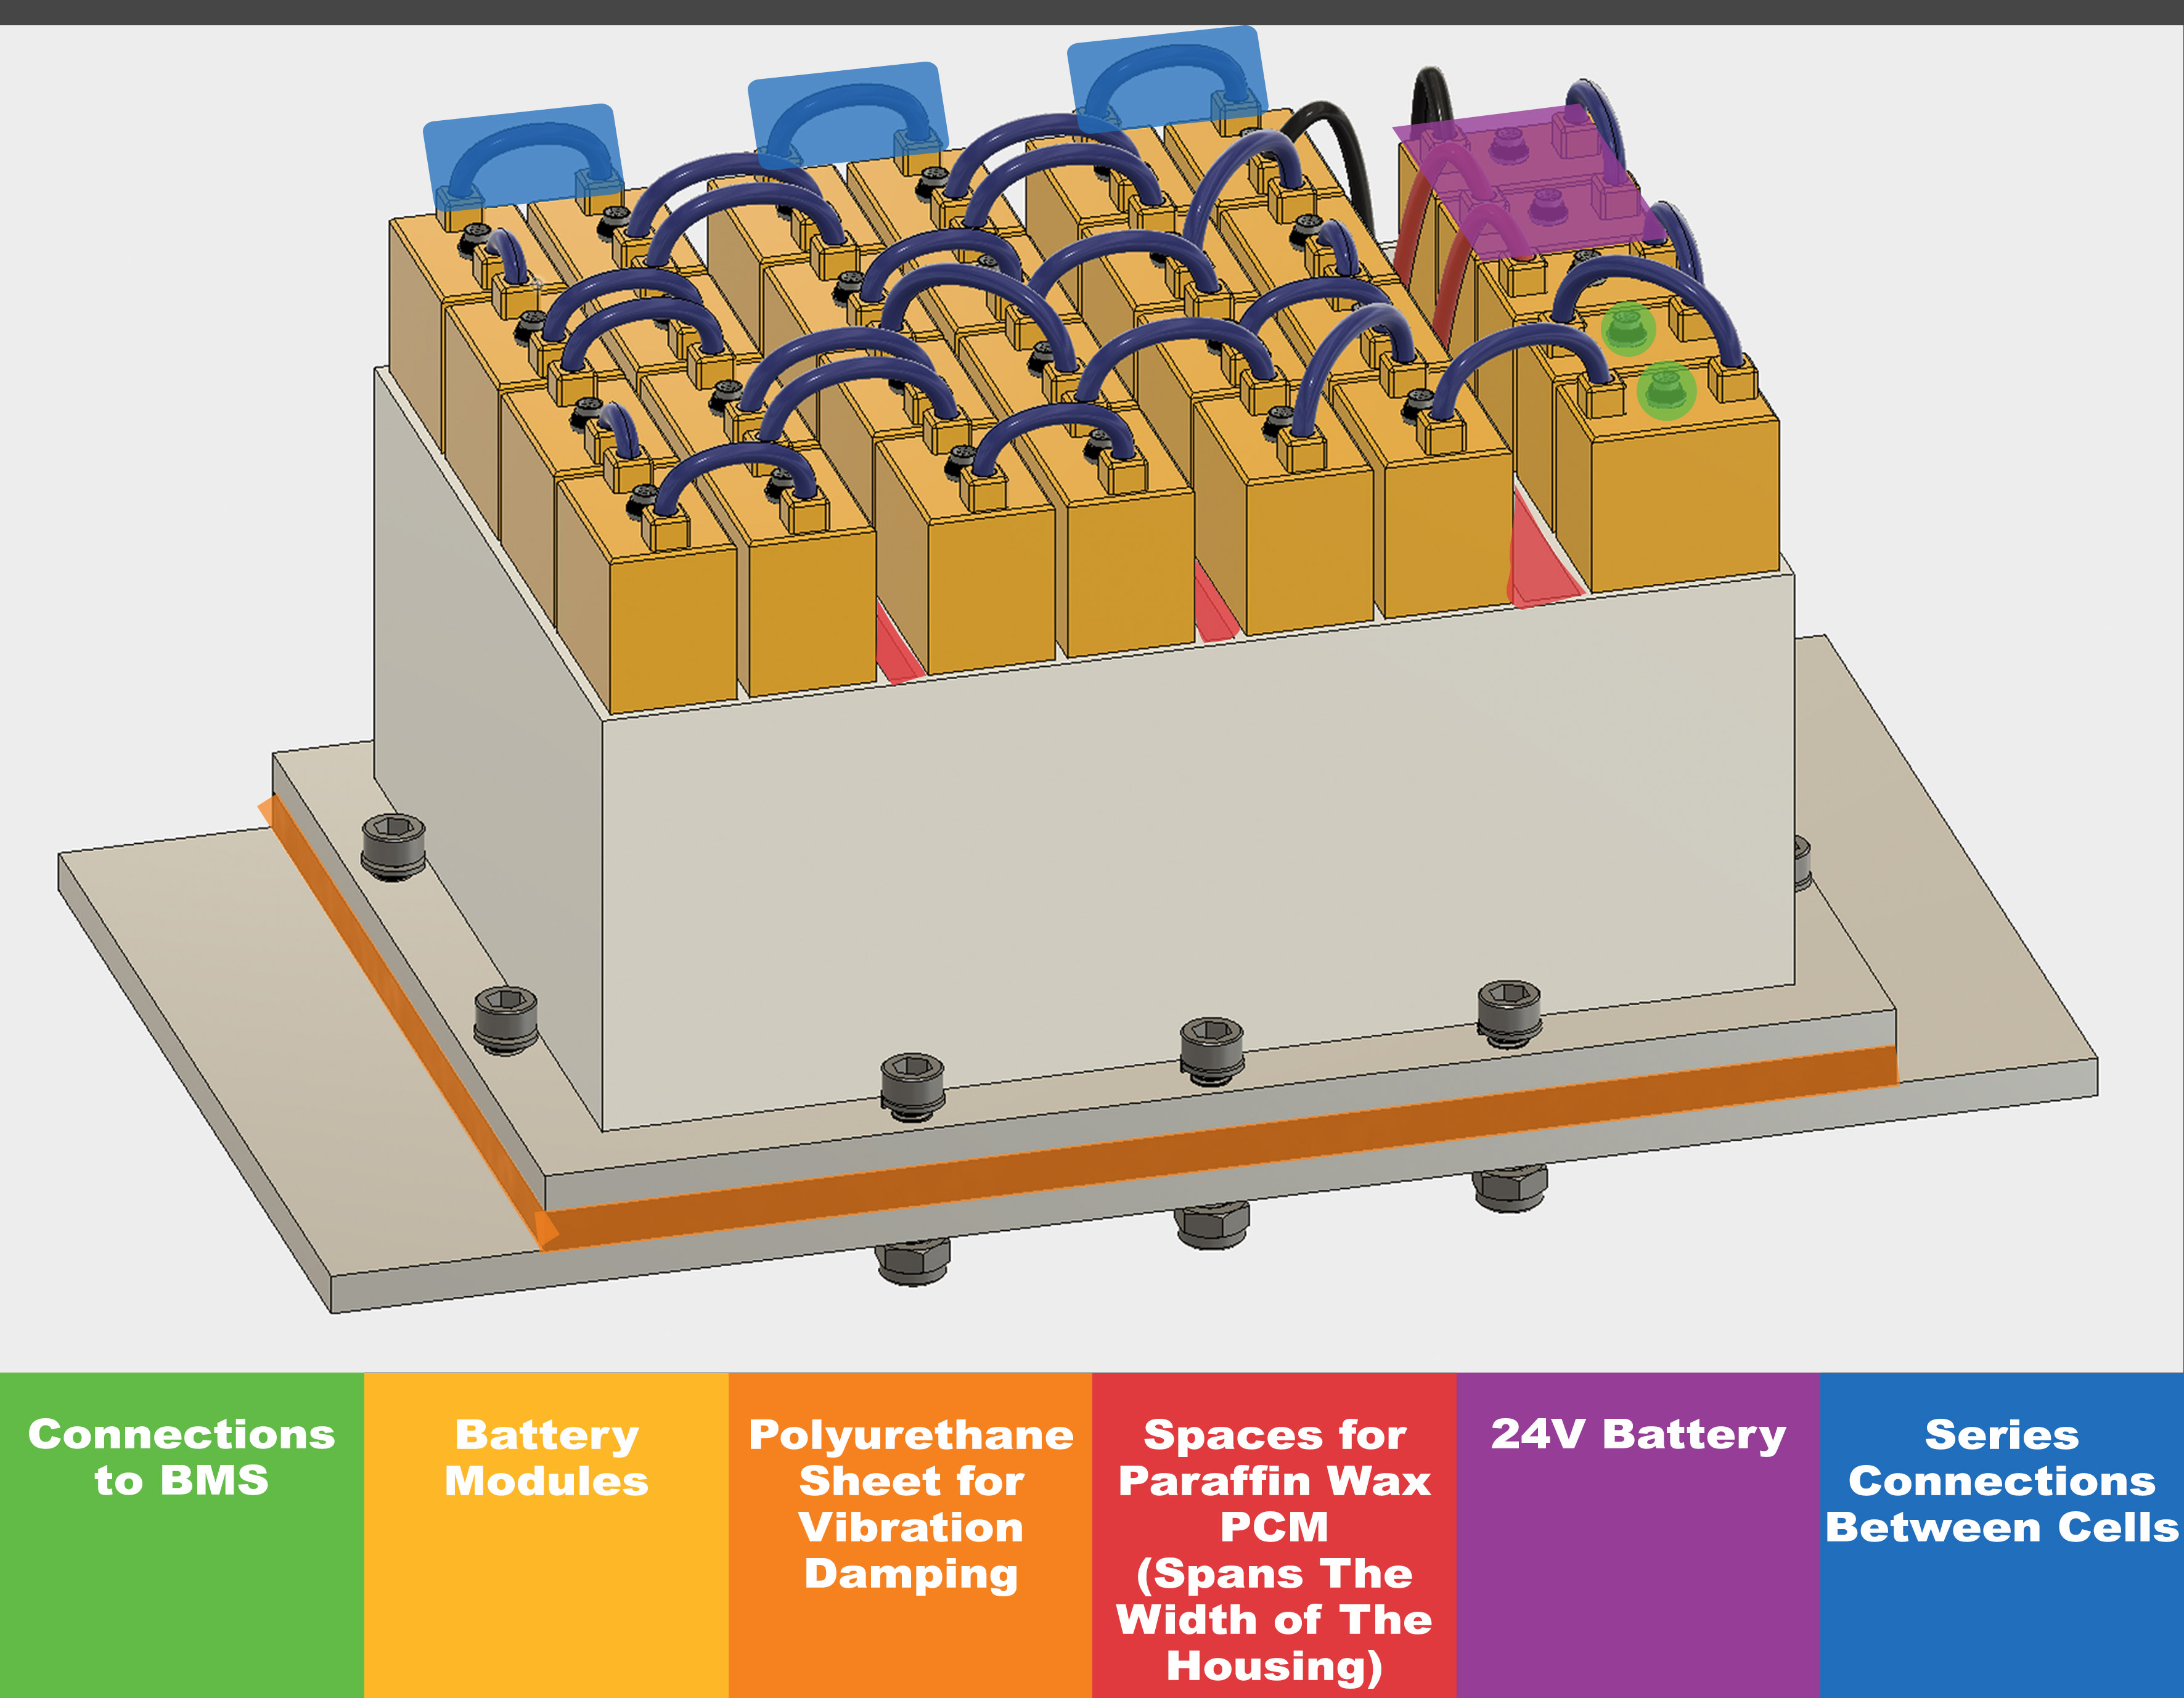
\includegraphics[width=\linewidth]{images/battery_description.jpg}

    \subsection{567V Battery}
    The 567V battery will be referred to as the "main battery" for the rest of this document.\\
    \begin{table}
        \centering
        \begin{tabular}{@{}lr@{}} \toprule
            Specification & Main Battery\\ \midrule
            Dimensions (L $\times$ W $\times$ H) & \SI{340}{mm} $\times$ \SI{208.5}{mm} $\times$ \SI{180}{mm}\\
            No. of Cells & 135 (\SI{567}{V}/\SI{4.2}{V})\\
            No. of Modules & 27 (135 cells, 5 cells per module)\\
            Voltage (peak) & \SI{567}{V}\\
            Voltage (nominal) & \SI{499.5}{V}\\
            Current (peak) & \SI{337.5}{A} (\SI{3.75}{Ah} $\times$ \SI{90}{C})\\
            Current (continuous) & \SI{168.75}{A} (\SI{3.75}{Ah} $\times$ \SI{45}{C})\\
            Internal Resistance &\SI{0.162}{\Omega} (\SI{0.0012}{\Omega} $\times$ \SI{135}{cells})\\
            Power (peak) & \SI{191}{kW} (\SI{337.5}{A} $\times$ (\SI{4.2}{V} $\times$ 135 cells))\\
            Power (continuous) & \SI{91}{kW} (\SI{168.75}{A} $\times$ (\SI{4}{V} $\times$ 135 cells))\\
            Capacity & \SI{3.75}{Ah}\\ \bottomrule
        \end{tabular}
        \caption{Main Battery Specifications}
        \label{tab:main-bat-specs}
    \end{table}
    
    LiPo cells were chosen to power the friction drive motor because of their ability to continuously discharge large amounts of current. This means that we don't have to connect any cells in parallel, cutting weight and saving money.\\
    
    To ensure that we have enough capacity for sufficient testing we will manufacture the housing to make installing/uninstalling the modules as easy as possible. This will allow us to replace and charge discharged modules with as little down time as possible.

    To achieve a voltage of 567V the main battery (see \reftab{tab:main-bat-specs} for specifications) will be an assembly of 27 modules (see \reftab{tab:module-specs} for specifications and \reffig{fig:module-model} for model). Each module housing 5 LiPo cells giving a total of 135 cells.\\

    Each cell (see \reftab{tab:cell-specs} for specifications and \reffig{fig:cell-model} for model) has a peak voltage of 4.2V and a capacity of 3750mAh. A high discharge rate of 90C (manufacturer spec) means the battery will be capable of supplying up to 337.5A.\\

    The 135 cells will be connected in series for a peak of \SI{567}{V} and \SI{337.5}{A}, meaning a maximum power of \SI{191}{kW}.\\
    
    This battery will be able to adequately power the main battery. The voltage of the battery was determined due to the minimum required voltage of \SI{467}{V} to achieve top speed. Accounting for voltage drop due to internal resistance, if the motor were operating at \SI{193}{A} or \SI{51}{C} (required current to achieve desired top speeds) would result in at \SI{31}{V} drop from the peak battery capacity of \SI{567}{V}. This sets the voltage range of each individual cell from approximately \SI{4.00}{V} - \SI{3.50}{V} in order to stay within desired speeds. Thus the total voltage of the battery pack will range from \SI{536}{V} - \SI{472.5}{V}. Based on approximate discharge curves for a LiPo cell at approximately \SI{50}{C}, the main battery should be capable of providing sufficient power to the Friction Drive over the approximately 12 second long acceleration. However further testing that is outlined later in this document will be required to validate these estimates, as discharge rates of LiPo cells will vary slightly from product to product.\\
    
     \begin{figure}[H]
        \centering
        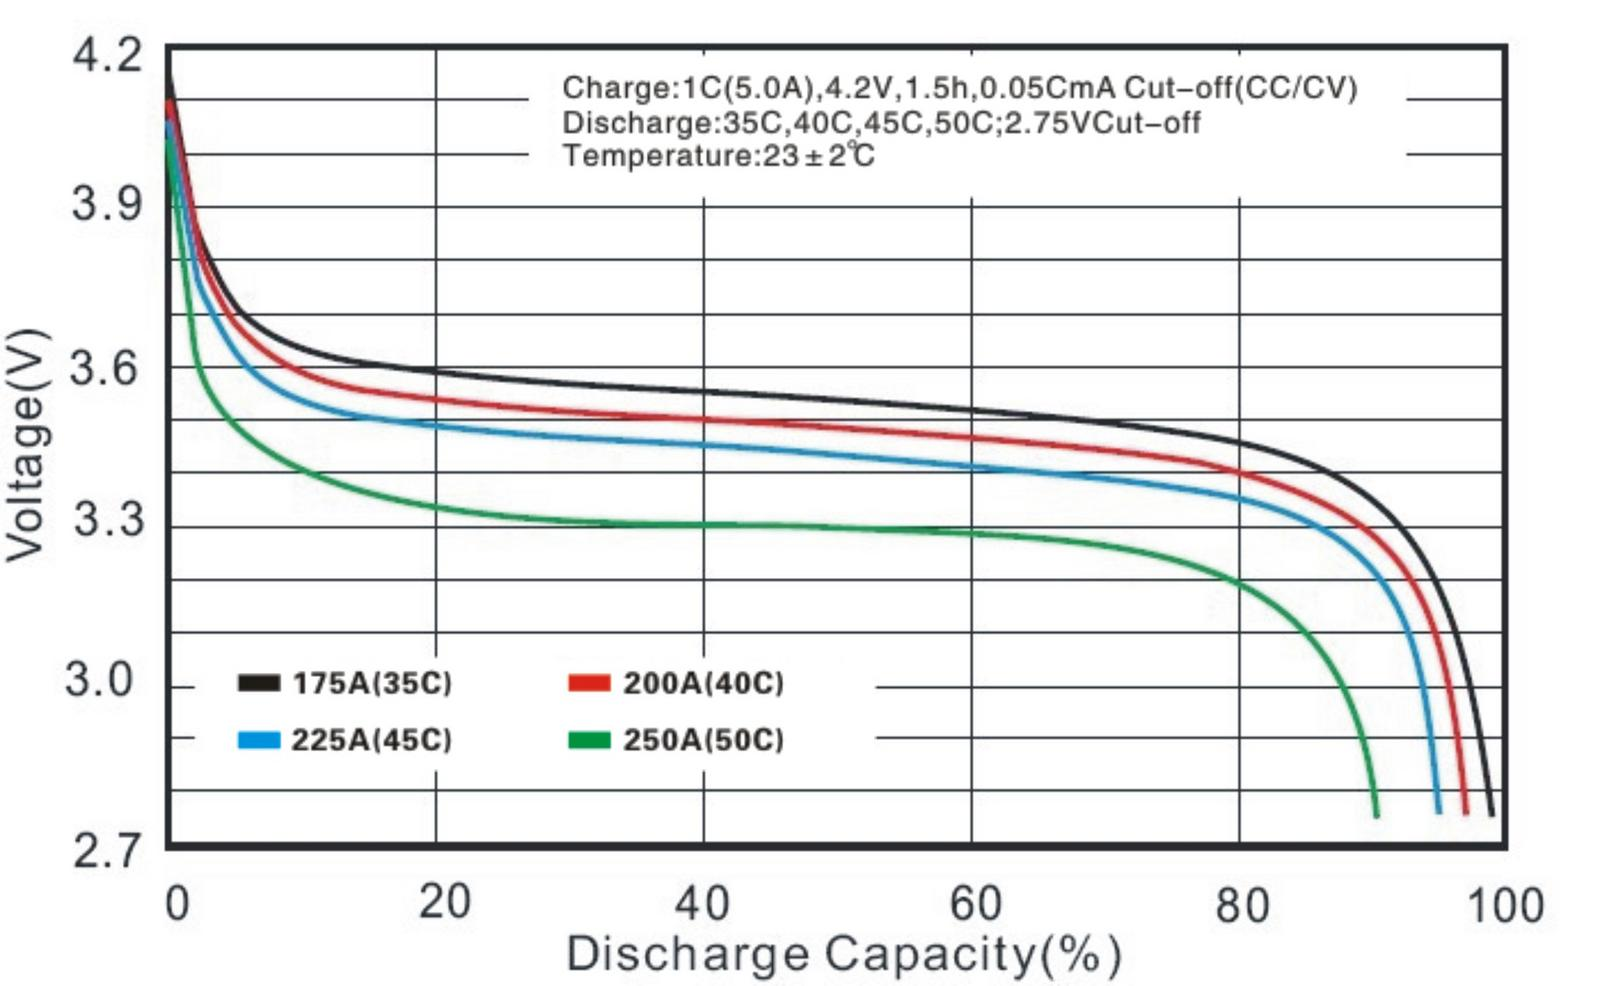
\includegraphics[width=\linewidth]{images/Discharge.jpg}
        \caption{Discharge Curve of a LiPo cell.}
        \label{fig:Discharge.jpg}
    \end{figure}
    
    \begin{figure}[H]
        \centering
        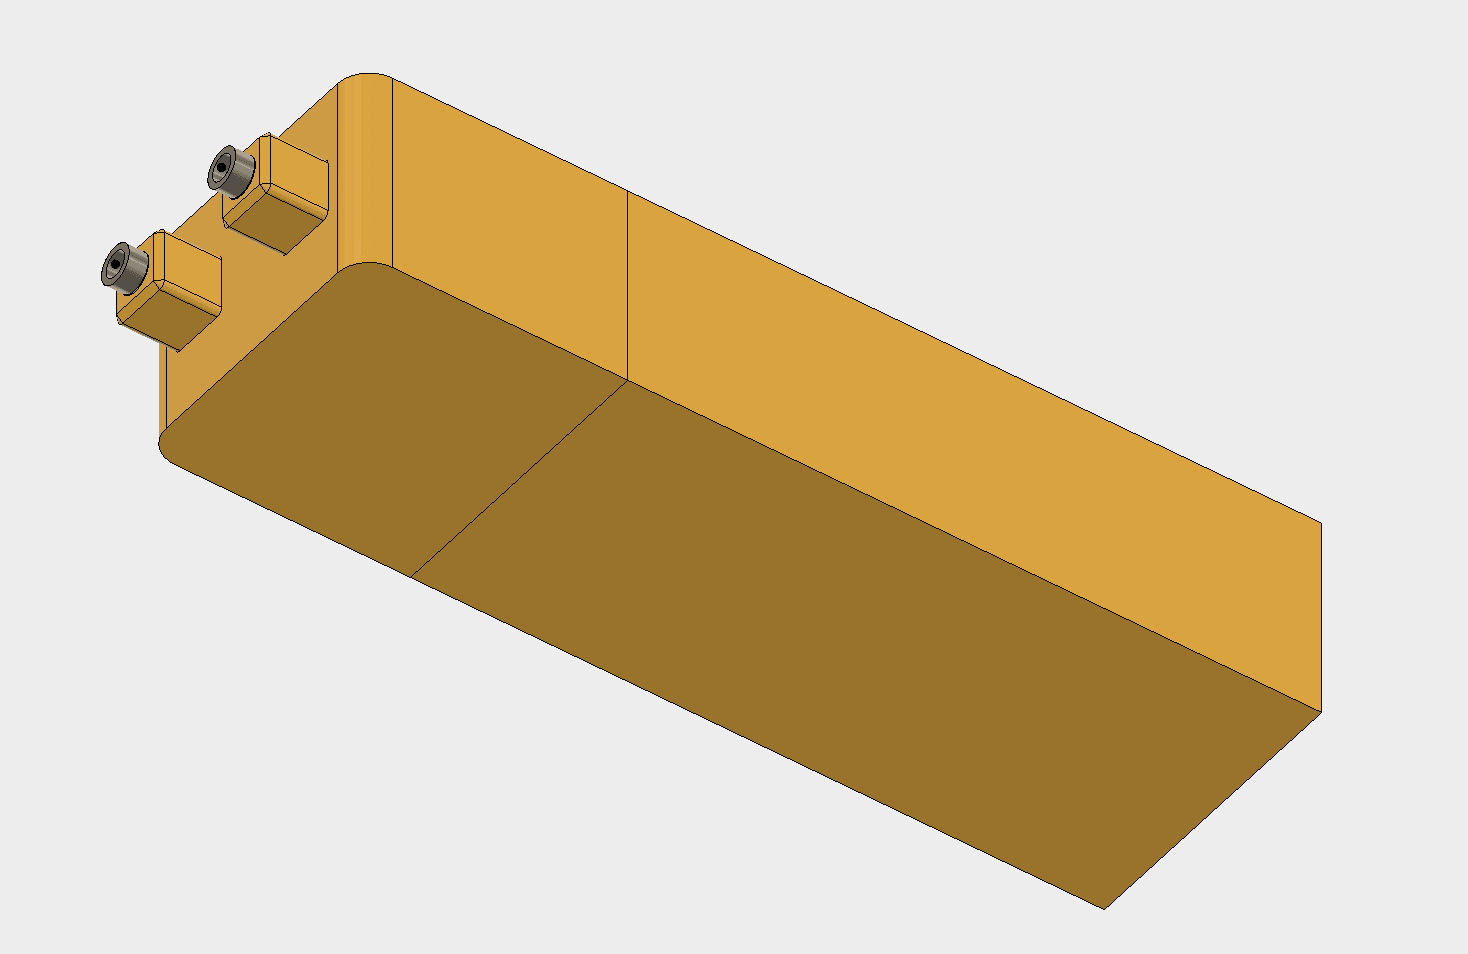
\includegraphics[width=\linewidth]{images/cell_module}
        \caption{Cell Module Model}
        \label{fig:module-model}
    \end{figure}
    
    \begin{table}[H]
        \centering
        \begin{tabular}{@{}lr@{}} \toprule
            Specification & Main Battery Module\\ \midrule
            Dimensions (L $\times$ W $\times$ H) & \SI{132.5}{mm} $\times$ \SI{47}{mm} $\times$ \SI{30.5}{mm}\\
            No. of Cells & 5 (\SI{567}{V}/\SI{4.2}{V})\\
            Voltage (peak) & \SI{21}{V} (\SI{4.2}{V} $\times$ 5 cells)\\
            Voltage (nominal) & \SI{18.5}{V} (\SI{3.7}{V} $\times$ 5 cells)\\
            Current (peak) & \SI{337.5}{A} (\SI{3.75}{Ah} $\times$ \SI{90}{C})\\
            Current (continuous) & \SI{168.75}{A} (\SI{3.75}{Ah} $\times$ \SI{45}{C})\\
            Internal Resistance &\SI{0.006}{\Omega} (\SI{0.0012}{\Omega} $\times$ \SI{5}{cells})\\
            Power (peak) & \SI{7}{kW} (\SI{337.5}{A} $\times$ (\SI{4.2}{V} $\times$ 5 cells))\\
            Power (continuous) & \SI{3.37}{kW} (\SI{168.75}{A} $\times$ (\SI{4}{V} $\times$ 5 cells))\\
            Capacity & \SI{3.75}{Ah}\\ \bottomrule
        \end{tabular}
        \caption{Module Specifications}
        \label{tab:module-specs}
    \end{table}
    
    \begin{figure}[H]
        \centering
        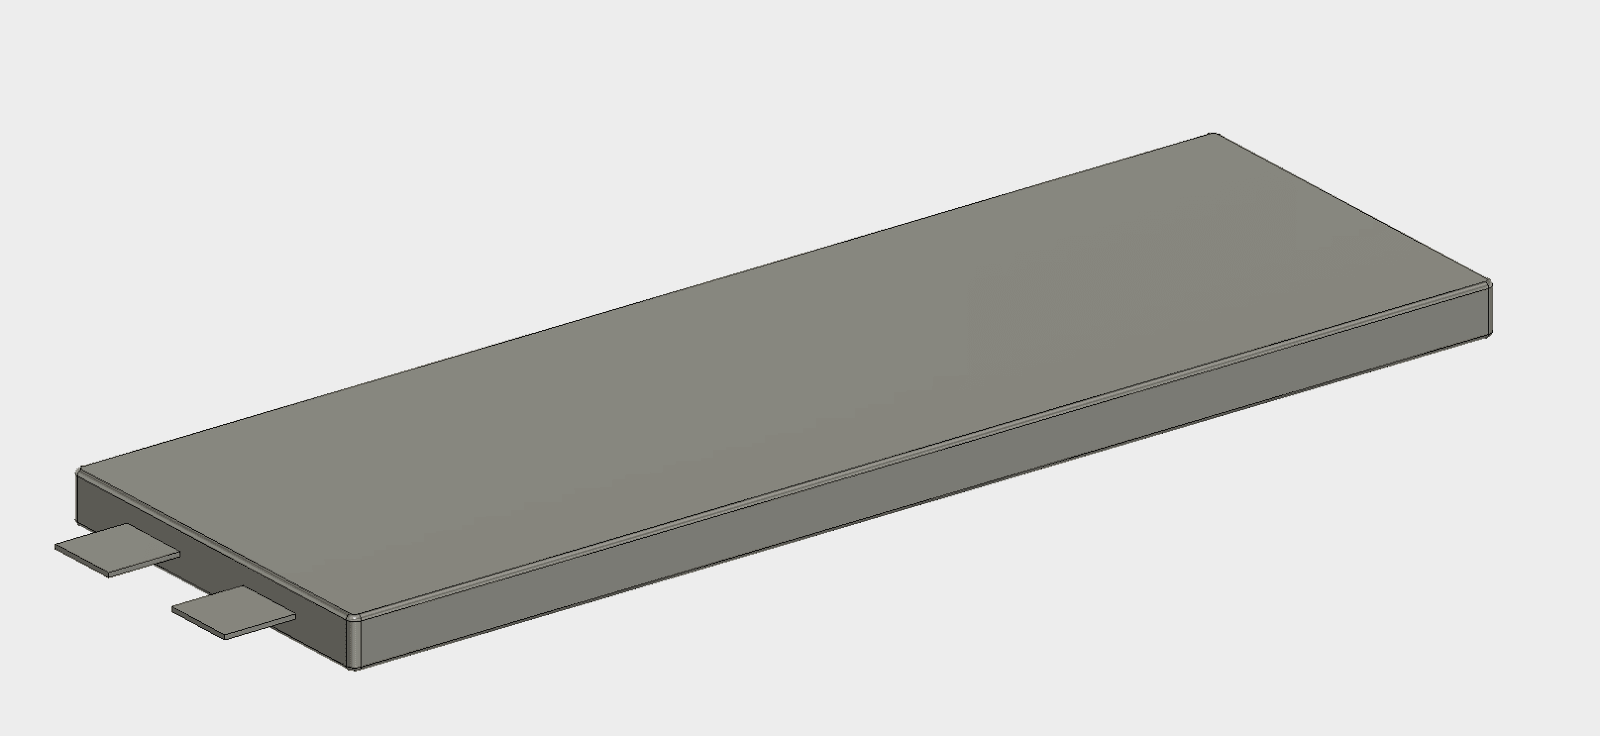
\includegraphics[width=\linewidth]{images/cell}
        \caption{LiPo Cell Model}
        \label{fig:cell-model}
    \end{figure}
    
    \begin{table}[H]
        \centering
        \begin{tabular}{@{}lr@{}} \toprule
            Specification & LiPo Cell\\ \midrule
            Dimensions (L $\times$ W $\times$ H) & \SI{128}{mm} $\times$ \SI{42.5}{mm} $\times$ \SI{5.4}{mm}\\
            No. of Cells & 5 (\SI{21}{V}/\SI{4.2}{V})\\
            Voltage (peak) & \SI{4.2}{V}\\
            Voltage (nominal) & \SI{3.7}{V}\\
            Current (peak) & \SI{337.5}{A} (\SI{3.75}{Ah} $\times$ \SI{90}{C})\\
            Current (continuous) & \SI{168.75}{A} (\SI{3.75}{Ah} $\times$ \SI{45}{C})\\
            Power (peak) & \SI{1.42}{KW} (\SI{337.5}{A} $\times$ \SI{4.2}{V})\\
            Power (continuous) & \SI{0.675}{KW} (\SI{168.75}{A} $\times$ \SI{4}{V})\\
            Capacity & \SI{3.75}{Ah}\\ \bottomrule
        \end{tabular}
        \caption{LiPo Cell Specifications}
        \label{tab:cell-specs}
    \end{table}
	
    \subsection{\textbf{\SI{24}{V}} Battery}
    \begin{table}
        \centering
        \begin{tabular}{@{}lr@{}} \toprule
            Specification & \SI{24}{V} Battery\\ \midrule
            Maximum Voltage & \SI{25.2}{V}\\
            Nominal Voltage & \SI{22.2}{V}\\
            Minimum Voltage & \SI{19.2}{V}\\
            Capacity & \SI{7.5}{Ah}\\
            Current Draw & \SI{5.19}{A}\\
            Power Draw & \SI{70.0}{W}\\
            Discharge Rate & \SI{0.69}{C}\\
            Time to Discharge & \SI{87}{mins}\\ \bottomrule
        \end{tabular}
        \caption{24V Battery Specifications}
        \label{tab:24V-bat-specs}
    \end{table}
    The \SI{24}{V} battery (see \reftab{tab:24V-bat-specs} for specifications) will be constructed of the same cells as the main battery. This decision was made to be resource and cost efficient, since designs and materials from the main battery can be carried over. The battery will be contained within the same housing as the main battery. The cell arrangement is 6S2P, and will be built from the same cells as the main battery. The \SI{24}{V} battery will power the embedded system, including all sensors (including ESC’s additional functions). In the instance the 24V battery fails, there will be a backup battery with identical specs, but with half the capacity (6S1P configuration). This backup battery will be held isolated from the other batteries in  a location identified in the sensor map (in embedded section). This location was chosen due to the short distance from friction and EC brakes, which would need to be activated in case of an emergency. The backup battery would immediately send a disengage the Friction Drive and engage EC brakes. The backup battery is essential since, if the main \SI{24} {V} battery failed, it would cause the friction brakes to engage at high speeds.
    \begin{table}[H]
        \centering
        \begin{tabular}{@{}lrrrrrc@{}} \toprule
            Component & Quantity & \makecell{Operating \\ Voltage (V)} & \makecell{Current \\ Draw/Unit (A)} & \makecell{Total Current \\ Draw (A)} & \makecell{Power \\ Draw (W)} & Notes\\ \midrule
            Arduino Mega & 4 & 5 & 0.05 & 0.2 & 1 &\\
            Raspberry Pi & 3 & 5 & 0.7 & 2.1 & 10.5 &\\
            Contact Temp. & 8 & 5 & 0.00005 & 0.0004 & 0.002 &\\
            IR Temp & 8 & 3.3 & 0.00024 & 0.00192 & 0.006336 &\\
            PED & 4 & 24 & 0.1 & 0.4 & 9.6 &\\
            IMU & 3 & 3.3 & 0.0016 & 0.0048 & 0.01584 &\\
            Tilt & 1 & 24 & 0.0015 & 0.0015 & 0.36 &\\
            Shaft Encoder & 1 & 7 & 0.05 & 1 & 0.35 &\\
            Liquid Pressure Sensor & 2 & 5 & 0.003 & 0.006 & 0.03 &\\
            Water Pump & 1 & 12 & 0.75 & 0.75 & 9 &\\
            Pressure Transducer & 2 & 24 & 0.04 & 0.08 & 1.92 &\\
            Pneumatic Solenoid & 6 & 24 & 0.1 & 0.6 & 14.4 &\\
            Reed Switch & 4 & 5 & 0.01 & 0.04 & 0.2 &\\
            ESC & 1 & 24 & 0.9 & 0.9 & 21.6 & \makecell{Inrush \\ current of 4A}\\ \midrule
            Total & & & & 5.15 & 68.99 &\\ \bottomrule
        \end{tabular}
        \caption{Power/Current Consumption of Components}
    \end{table}
    
 \begin{table}[H]
        \centering
        \begin{tabular}{@{}lrr@{}} \toprule
            \makecell{Operating \\ Voltage (V)} & \makecell{Current \\ Draw (A)}  &  \makecell{Power \\ Draw (W)} \\ \midrule
            24 & 2.04 & 48.04\\
            12 & 0.75 & 9 \\
            5 & 2.31 & 11.55 \\
            3.3 & 0.01 & 0.02 \\
        \end{tabular}
        \caption{Power Consumption of Each Operating Voltage. As seen in table 24V systems drew the most power, which led to the selection of a 24V battery, to reduce power lost as heat when regulating voltage.}
    \end{table}
    \paragraph{Wire Management}
    The wire used to power the motor needs to support a voltage of \SI{625}{V} and a current of \SI{205}{A}. This will need to run from the battery to the motor, which are about \SI{0.5}{m} apart from each other. According to guidelines outlined by Blue Sea Systems Inc.\footnote{“Part 1: Choosing the Correct Wire Size for a DC Circuit.” Internet: https://www.bluesea.com/resources/1437, May 19, 2010 [Dec 17, 2017]}, this wire needs to be a 2|0 AWG copper wire. The arduinos and sensors do not require a current greater than \SI{5}{A}, so they can use 16 AWG copper wire.\\

    Wires will be routed such that power lines for main battery will be as far away as possible from all other cables to avoid interference. In addition, the wires will be shielded to prevent interference from external magnetic fields. To reduce the number of free wires, connections joining similar locations will be held together using a polyester plastic sleeving. Wires running the length of the pod will be fastened to the pod with a PVC wire duct that is screwed to the frame. Wires providing a current of less than \SI{9.0}{A} will be connected using the Mini-Fit Jr. connectors by Molex.  Connections that need to support greater currents will use 6 pin circular mic connectors.


    \subsection{Battery Management System}
    \paragraph{Main Battery}
   	The main battery will use Elithion's Lithiumate Pro BMS, which monitors voltage and current output, as well as the temperature of each cell. The Lithiumate Pro is often used by electric vehicle enthusiasts, so it is a highly reputable system. 
    
    The BMS is being supplied by Elithion, who has a reputation for building reliable Battery Management Systems for many different prototypes and student design teams.
    

     \begin{figure}[H]
        \centering
        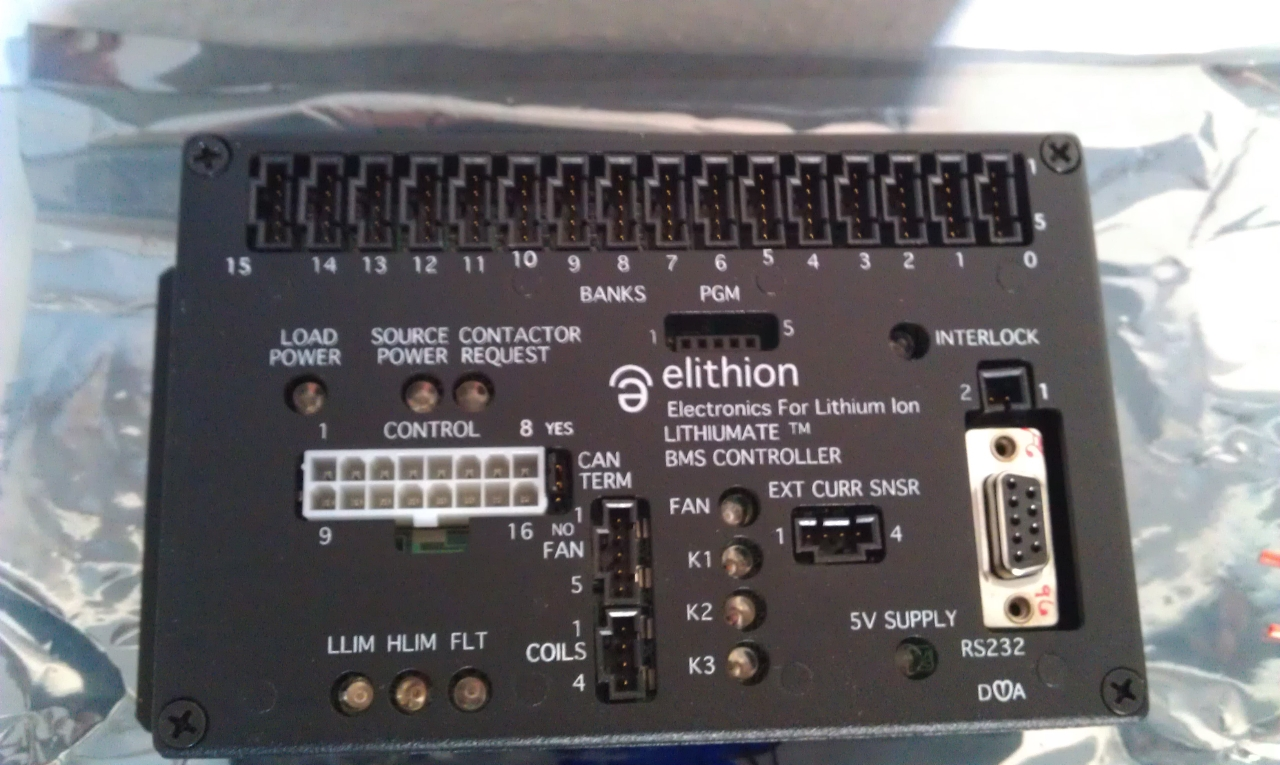
\includegraphics[width=\linewidth]{images/lithiumate_pro}
        \caption{The Lithiumate Pro BMS Master}
        \label{fig:bms-master}
    \end{figure}   
 
 	The BMS master above connects to the cells via "cell boards".  Cell boards measure the voltage and temperature measurement of each cell. There are 16 ports on the BMS which connect to strings of cells daisy-chained together - in our case, we'll have 15 strings of 10 cells and one of 5 (135 cells in total). The cell boards will be put inside the modules as shown in the following exploded view of the battery module. We'll have 2 modules per string (except the last one) as each module only holds 5 cells.
     
     \begin{figure}[H]
        \centering
        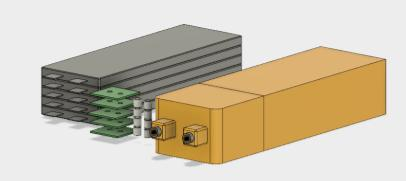
\includegraphics[width=\linewidth]{images/ExplodedModule}
        \caption{Exploded Cell Module With BMS Cell Boards (green) and Spacers Visible}
        \label{fig:exploded-cell}
    \end{figure}
     
	The BMS will also come with a current sensor to ensure we are drawing the correct amount of current.
	The Lithiumate Pro can communicate via the CAN bus, so that's how the important battery information will be sent to the on-board computers for analysis.     
     
    \paragraph{24V Battery}
	The 24V battery will use a commercially available 6S BMS. In order to ensure the BMS works as advertised, basic tests will be conducted (e.g. try to draw current above what BMS is restricted to).
    
	\subsection{Battery Charging}
    \paragraph{Main Battery} 
	The modules of the main battery will be disconnected and charged individually, eliminating the need for a high voltage battery charger. Individual 21V (4.2V x 5 cells) chargers will be used to charge the modules of the battery.
    \paragraph{24V Battery}
    The 24V battery will be charged using off the shelf LiPo cell chargers, which are already owned by the team.
    
    ESC, how power will be transferred and ensured for safety

    \section{Failsafes}
    In the event of an electrical systems failure, precautions have been taken to ensure the pod will respond in a safe, controlled and repeatable fashion. The following sections describe how critical subsystems like the friction drive, braking systems, and embedded control hardware handle an electrical failure.
    \subsection{Battery}
    The three main power sources on the pod are the high voltage battery for the friction drive, the 12V battery for powering software and braking functionality, and a backup 12V for redundancy.  If the main battery stops functioning, the EC brakes will activate, and the software system will safely bring the pod to a stop (by engaging friction brakes at speeds lower than 10 m/s). If one of the 12V batteries stops functioning, the EC brakes will activate, and the other battery will continue to power the Arduinos and sensors. To avoid a loss of power to software during the battery switch, a capacitor connected in parallel will briefly supply the current for the Arduino hubs. Once the EC brakes are activated, the software system will safely bring the pod to a stop. The battery failsafe circuit is pictured in ---------> MISSING FIGURE <---------, and all the outcomes are listed in \reffig{tab:efailsafe}. In the table, it is important to note that a status of 1 represents a voltage present. Since the friction brakes and EC brakes are in a normally closed state, they are engaged when their status is 0.
    
\begin{table}[H]    
\centering
\begin{tabular}{@{}ccc|ccccc@{}} \toprule
%\hline
\multicolumn{3}{c}{Input} &  & \multicolumn{4}{c}{Output}                                    \\ 
\midrule
Main Battery & 12V 1 & 12V 2 &  & All Arduino Hubs & EC Brakes & Friction Brakes & Friction Drive \\ \midrule
1            & 1     & 1     &  & 1                & 0         & 1               & 1              \\
1            & 1     & 0     &  & 1                & 1         & 1               & 0              \\
1            & 0     & 1     &  & 1                & 1         & 1               & 0              \\
0            & 1     & 1     &  & 1                & 1         & 1               & 0              \\
0            & 1     & 0     &  & 1                & 1         & 1               & 0              \\
0            & 0     & 1     &  & 1                & 1         & 1               & 0              \\
\bottomrule
\end{tabular}
\caption{Battery Failsafe Truth Table}
\label{tab:efailsafe}
\end{table}

    \begin{figure}[H]
        \centering
        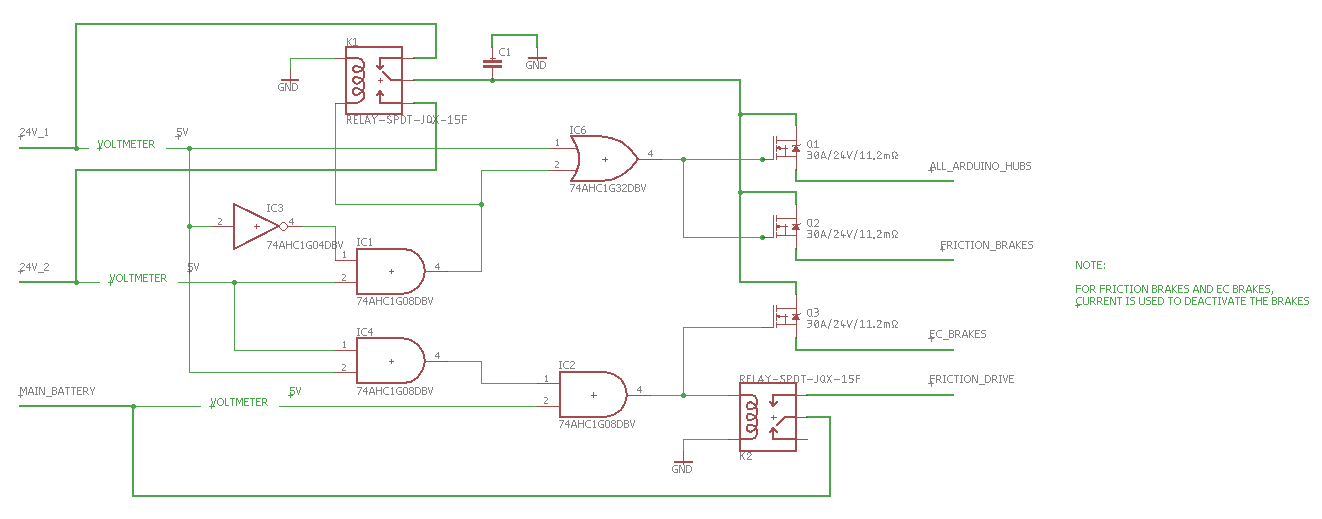
\includegraphics[scale = 0.5]{images/Failsafe}
        \caption{Electrical Failsafe Circuit }
        \label{Failsafe}
    \end{figure} 
    
    \begin{figure}[H]
        \centering
        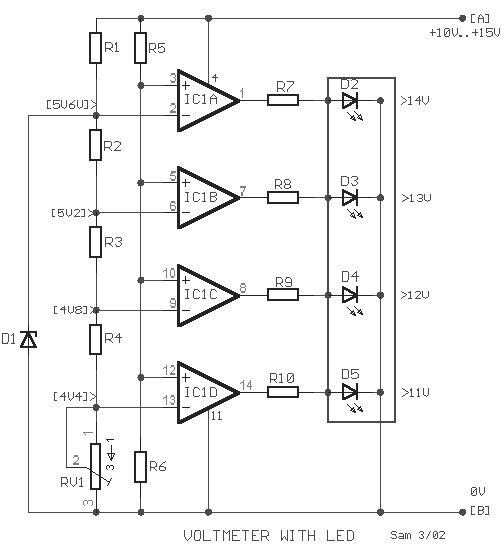
\includegraphics[scale = 0.5]{images/Voltmeter}
        \caption{Voltmeter circuit from Electrical Failsafe Circuit}
        \label{Voltmeter}
    \end{figure} 
    
    \subsection{BMS}
    One of the pod safety specfications stipulated by SpaceX is the isolation of the battery during overtemperature conditions.The cell boards output a temperature reading that is measured by the BMS master. An overtemperature condition will result in a fault being set on the CAN bus. Once the fault is observed from the on board computer, the battery is galvanically isolated via a contactor switch, as shown in \reffig{fig:contactor}. The EVC 250-800 is an automotive grade contactor manufactured by TE Connectivity, and is rated for 800V and 250A (continuous).
    \begin{figure}[H]
        \centering
        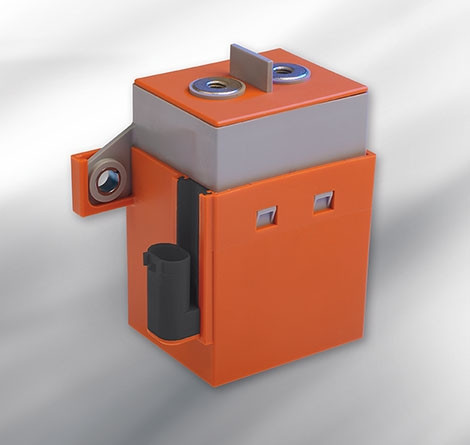
\includegraphics[scale = 0.5]{images/contactor}
        \caption{TE Connectivity EVC 250-800 - Automotive Contactor }
        \label{fig:contactor}
    \end{figure}  
    
    \subsection{Inhibits on Braking During Acceleration}
    A critical safety feature is the prevention of braking during the pod's acceleration phase. The primary failure mode for this situation would be the cutoff of current flow to the solenoids that hold the brakes (EC or friction) in the disengaged position. Potential failure mechanisms include a faulty connection or wire, or the control relay that enables current flow failing open. Both braking mechanisms have reed switch sensors which will inform the embedded computer of the brake's position. If the brakes become engaged during the acceleration phase, the control software can disable the friction drive.


    
    
    \section{Testing}
    Since different cell chemistries (even similar ones) react differently to various incidents (i.e. puncturing the cell), it was determined that the most effective way to show the battery design will be safe would be to experimentally test various components of the batteries to varying  extents, and using experimentally derived results to determine safe operating ranges for the batteries. The 3.7 V batteries used as backup power for the Arduino and Raspberry Pi have already been tested previously by our team in a vacuum, drawing expected current draw with no issues. Outlined in \refsec{subsec:testing-proc} are general testing plans for the main and 24V battery. They will be furthered expanded upon once details of testing have been finalized.
    \subsection{Purpose of Testing}
    To determine the absolute limits of batteries and to determine expected range of values for battery including temperature, current, and voltage under various different conditions.
    \subsection{Parameters of Testing}
    All cell level testing (testing levels will be described later further on) will be done to failure with the exception of vacuum testing (in order to protect testing equipment). With the exception of vibration testing, module level testing will be tested to failure with the exception of vibration testing, which will be done through a wide range of frequencies. The final battery will undergo no destructive testing however testing from all level testings should provide a thorough analysis of how final battery will react to various different unexpected scenarios.
    \subsection{Equipment for Testing}
    Temperature sensors (both IR and contactless) will be used to monitor temperature of batteries in all tests. A shunt resistor and arduino will be used to measure current and voltage at all times, in all tests. Impact testing and hydraulic press testing will most likely be performed at university facilities, however facilities have not been confirmed. Vibration testing will be performed at Infinity Testing Solutions, however use of facilities for Goose III have not been confirmed.
    \subsection{Testing Procedure}
    \label{subsec:testing-proc}
    Side Note: Testing will be broken into three “levels”; cell testing, module testing and battery testing. This testing is specifically with regards to the 535V battery. While the other batteries (24V and 3.7 V) will be tested, the 535V battery will be tested to the most rigorous degree, as a failure of this battery would lead to a significantly more catastrophic outcome than the other ones.

    \paragraph{Level One: Cell Testing}
    This level of testing is where the most destructive testing will occur, since cells are relatively cheap in comparison to modules and the full battery. The cells being tested on will be from the Turnigy’s Nano-tech Ultimate  7500 mAh 2S2P. Since the battery comes in a variety of different capacities, all cell level testing will be done on both the 3750 mAh cells as well as the 1300 mAh cells, to determine the consistency of the specific cell chemistry. This will help the team, in the instance our power demands change and a change in capacity is required. The cell level tests include:
    \begin{enumerate}
        \item \textbf{Mechanical Damage}
        \begin{enumerate}
            \item \textit{Impact Testing}
            \begin{enumerate}
                \item \textbf{What: }Use impact testing facilities to expose the cells to impulses of increasing values, until failure.
                \item \textbf{Why: }To understand what precautions need to be taken while transporting the batteries, whether this is driving the battery to competition, what to expect if the battery is accidentally dropped, and any other potential cases that may damage the battery.
                \item \textbf{Recorded Data: }Qualitative analysis (including video) and maximum impulse a cell can handle from various angles.
                \item \textbf{Next steps: }To model the full battery based on the results from cell testing.
            \end{enumerate}
            \item \textit{Puncture Testing}
            \begin{enumerate}
                \item \textbf{What: }Use a nail to puncture the cells in various locations.
                \item \textbf{Why: }To understand what will happen if cell is accidentally punctured during assembly or transport. This case will realistically not occur once the battery is assembled, thus will only be of importance to those involved in battery assembly.
                \item \textbf{Recorded Data: }Qualitative analysis (including video) and heat generated over time.
                \item \textbf{Next Steps: }N/A
            \end{enumerate}
        \end{enumerate}
        \item \textbf{Over Current Damage}
        \begin{enumerate}
            \item \textbf{What: }Short the two leads of the battery together in a safe environment.
            \item \textbf{Why: }To understand what will occur in case of a short, since various LiPo cells  react differently when shorting (some, just gas, while others start a fire).
            \item \textbf{Recorded Data: }Qualitative analysis (including video), maximum dimensions of cell (via video analysis) and heat generated.
            \item \textbf{Next Steps: }Model the full battery overcurrent damage based on data from cell damage.
        \end{enumerate}
        \item \textbf{Over Charging Damage}
        \begin{enumerate}
            \item \textbf{What: }Charge cell to increasing levels of voltage above 4.2 V max charge rating.
            \item \textbf{Why: }To test the maximum manufacturer rating for the battery, and to see how far above it the battery can go (or if it is even capable of reaching 4.2 V). Batteries used in competition will not be charged about maximum manufacturer rating nor will they have been previously charged above this value. The overcharge component of the test is purely for testing purposes.
        \end{enumerate}
        \item \textbf{Cycle Testing}
        \begin{enumerate}
            \item \textbf{What: }Cycle cells at various discharge rates, including and above our expected discharge rate.
            \item \textbf{Why: }To determine the expected life cycle of the full battery. If our battery is used for different purposes in the future, expected lifespan can then be calculated from tests at different discharge rates. Furthermore, this will help determine whether or not the battery manufacturer’s listed specs are valid.
            \item \textbf{Recorded Data: }Qualitative analysis (including video), cell charge and discharge rates and times, charge capacity, heat generation, and cell initial and final dimensions (plus any other notable dimension changes if any).
            \item \textbf{Next Steps: }N/A
        \end{enumerate}
        \item \textbf{Vacuum Testing}
        \begin{enumerate}
            \item \textbf{What: }High current testing in a vacuum up to 90C or until it appears (both qualitatively and thermally) the cell is about to explode. This test must be conducted last of the five cell level tests. While the order of other tests does not matter, this test must be conducted last. The data of the other tests will provide expected ranges in which the battery can safely operate (i.e. temperature, expansion, etc.). There must be automatic shutoffs in place when any value exceeds safe ranges in order to avoid damaging the testing facility.
            \item \textbf{Why: }To ensure the battery will operate safely in a vacuum, while drawing a high current, since pressure changes may cause increase expansion rate.
            \item \textbf{Recorded Data: }Qualitative analysis (including video), current and voltage draw,
            \item \textbf{Next Steps: }If cells do expand due to testing, determine whether or not the cells can be safely used in the design, or if new cell needs to be used
        \end{enumerate}
    \end{enumerate}
    \paragraph{Level Two: Module Testing}
    This level of testing will be conducted on modules (4S). The cells being tested on will be from the Turnigy’s Nano-tech Ultimate  7500 mAh 2S2P. Since the battery comes in a variety of different capacity’s, all cell level testing will be done on both the 3750 mAh cells as well as the 1300 mAh cells (if time and budget permits), to determine the consistency of the specific cell chemistry. This will help the team, in the instance our power demands change and a change in capacity is required. The module level tests include:
    \begin{enumerate}
        \item \textbf{Expansion Testing}
        \begin{enumerate}
            \item \textbf{What: }Allow x number of cells (where x ranges from 1-4) to expand via a short circuit.
            \item \textbf{Why: }To determine what will happen in the instance a cell (or multiple cells) within a module expand.
            \item \textbf{Recorded Data: }Qualitative analysis (including video), and thermal analysis.
            \item \textbf{Next Steps: }Design and test multiple different module enclosures, to determine the safest, effective design.
        \end{enumerate}
    \end{enumerate}
    \paragraph{Level Three: Full Battery Testing}
    This level of testing will be conducted with the full battery (650V), in its completed arrangement. There will be no destructive testing at this level (due to cost), and data provided from previous tests should set parameters at which the battery can safely operate. The data from this level of testing should correlate with results from previous tests, however the current draw will be incrementally increased to avoid damage from unexpected factors. The first two tests will be conducted with a large number of temperature sensors (and potentially a thermographic camera) to create a simulated “map” of the battery’s temperature at any given location. From there the 3-4 points that have the tendency to be the hottest will chosen for the final sensor setup. The latter two tests will only use this 3-4 points of temperature monitoring, and will be conducted at competition using SpaceX’s vacuum facilities.
    \begin{enumerate}
        \item \textbf{Motor No Load Testing}
        \begin{enumerate}
            \item \textbf{What: }Incrementally increasing current draw from motor, until at max expected draw of 55C.
            \item \textbf{Why: }To ensure the motor, BMS, and ESC all work in conjunction with one another.
            \item \textbf{Recorded Data: }Qualitative analysis (including video), thermal profile, RPM of motor, and any other info the ESC and BMS will provide.
            \item \textbf{Next Steps: }N/A
        \end{enumerate}
        \item \textbf{Motor With Load Testing}
        \begin{enumerate}
            \item \textbf{What: }Once friction drive has been assembled and both the friction drive and battery have been integrated, the same test as the previous test will be conducted. If there is a test track available, there will be a second component to this test in which the pod will move down the racetrack.
            \item \textbf{Why: }To ensure the friction drive has been assembled correctly, and will function as expected.
            \item \textbf{Recorded Data: }Qualitative analysis (including video), and all sensor info from embedded system.
            \item \textbf{Next Steps: }N/A
        \end{enumerate}
        \item \textbf{Vacuum Testing}
        \begin{enumerate}
            \item \textbf{What: }Test the battery (with electronics powered on) within SpaceX’s vacuum testing facility.
            \item \textbf{Why: }To ensure everything works as expected.
            \item \textbf{Recorded Data: }Data from embedded systems.
            \item \textbf{Next Steps: }N/A
        \end{enumerate}
        \item \textbf{Motor Testing in Vacuum}
        \begin{enumerate}
            \item \textbf{What: }Test the pod down SpaceX’s race track.
            \item \textbf{Why: }To ensure everything works as expected.
            \item \textbf{Recorded Data: }Data from embedded systems.
            \item \textbf{Next Steps: }N/A
        \end{enumerate}
    \end{enumerate}
    \paragraph{General Next Steps (this includes tests marked N/A)}
    An initial Battery Safety 101 will be conducted with all members who participate in testing. Furthermore, all results from level one and two testing will be incorporated into a secondary Battery Safety Training which provide all necessary info on what to do with a cell, module or battery in any given instance.Training will be given to all members involved in battery construction, as well as the Integration leads. If at any point of testing, the batteries are deemed to be “too dangerous” (i.e. vacuum testing shows that cells will burst when drawing expected discharge rate of 55C), the team must go back to the drawing board and determine a new potential cell candidate.

\end{document}
